    \documentclass[12pt,a4paper]{article}
    \usepackage[T2A]{fontenc}
    \usepackage[utf8]{inputenc}
    \usepackage[russian]{babel}
    \usepackage{amsmath}
    \usepackage{amssymb}
    \usepackage{graphicx}
    \usepackage{floatrow}
    \usepackage{booktabs}
    \usepackage{wrapfig}
    \usepackage{lipsum}
    \usepackage{subcaption}
    \usepackage{fancyhdr}
    \usepackage{mathrsfs}
    \usepackage{tikz}

    \usepackage{graphicx, scalerel}
    \usepackage[warn]{mathtext}
    \usepackage{indentfirst}
    \usepackage[margin = 25mm]{geometry}
    \usepackage{caption}
    \usepackage{multirow}
    \usepackage{gensymb}
    
    \newcommand{\figref}[1]{(См. рис. \ref{#1})}
    \newcommand{\secref}[1]{(См. раздел. \ref{#1})}
    
    \newcommand{\e}[1]{\text{$\cdot10^{#1}$}}
    
    \pagestyle{fancy}
    \fancyhead{}
    \fancyhead[L]{Работа 5.2.2}
    \fancyhead[R]{}
    \fancyfoot[C]{\thepage}
    
    \author{\normalsize Выполнил: Голубович Тимур, группа Б01-110 \\
    	\normalsize 06.09.2023}
    \date{}
    
    \usepackage{float}
    \restylefloat{table}
    \title{
    	\large Отчет о выполнении лабораторной работы 5.2.2 \\
    	\Large Изучение спектров атомов водорода и молекулы йода
     }
    
    \begin{document}
    	\maketitle
    	
    \section*{Цель работы}
    Исследовать спектральные закономерности в оптическом спектре водорода. По результатам измерений вычислить постоянную Ридберга для водорода.
    
    \section*{Оборудование и приборы} 
    He-Ne-лазер; интерферометр Майкельсона с подвижным зеркалом; фотодиод с усилителем; осциллограф; поляроид; линейка.

	
    \section*{Теоретическое введение}

    \subsection*{Изучение спектра атома водорода}

	Атом водорода является простейшей атомной системой; для него уравнение Шредингера может быть решено точно. Поэтому спектр атома водорода является предметом тщательного экспериментального и теоретического исследования.
	
	Объяснение структуры спектра излучения атомов требует знания схемы атомных энергетических уровней, что, в свою очередь, требует решения задачи о движении электрона в эффективном поле атома. Для атома водорода и водородоподобных (одноэлектронных) атомов определение энергетических уровней значительно упрощается, так как квантово-механическая задача об относительном движении электрона (заряд $-e$, масса $m_e$) и ядра (заряд $Ze$, масса $M$) сводится к задаче о движении частицы с эффективной массой $\mu = m_e M/(m_e + M)$ в кулоновском поле $-Ze^2/r$. Однако даже для водородоподобных атомов это решение не является простым.

	
	Длины волн спектральных линий водородоподобного атома описываются формулой
	\begin{equation}
		\frac{1}{\lambda_{mn}} = RZ^2\left(\frac{1}{n^2} - \frac{1}{m^2}\right),
	\end{equation}
	
	\noindent где $R$ -- константа, называемая постоянной Ридберга, а $m$ и $n$ -- целые числа. Эта формула достаточно правильно описывает экспериментальные значения линий водорода при $R = 109 677,6$ см$^{-1}$.
	
	В данной работе изучается серия Бальмера, линии которой лежат в видимой области. Для серии Бальмера $n = 2$. Величина $m$ для первых четырех линий этой серии принимает значение $3, 4, 5, 6$. Эти линии обозначаются символами $H_\alpha$, $H_\beta$, $H_\gamma$, $H_\delta$.
	
	Энергия уровня с квантовым числом $n$ определяется формулой:
	\begin{equation}
		E_n = -\frac{m_e Z^2 e^4}{2\hbar^2}\frac{1}{n^2} = -R\frac{Z^2}{n^2}.
	\end{equation}

    \subsection*{Изучение молекулярного спектра йода}

 	\begin{figure}[h!]
		\centering
		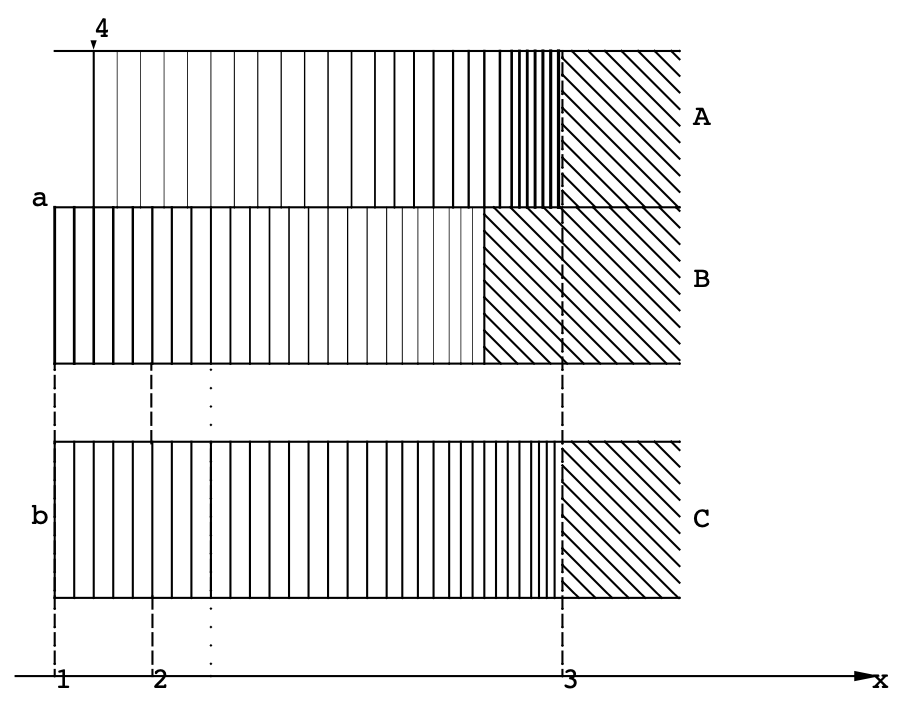
\includegraphics[width=10cm]{src/iodine.png}
		\caption{Спектр поглощения йода}
        \label{fig:iodine}
	\end{figure}
 
	Массы ядер атомов велики по сравнению с массой электрона. Благодаря такой разнице в массах, скорости движения ядер в молекуле малы по сравнению со скоростями электронов. Это даёт возможность	рассматривать электронное движение при неподвижных ядрах, расположенных на определенных расстояниях друг от друга. Определяя уровни энергии такой системы, мы найдем электронные термы молекул. Любой атом в молекуле находится в электрическом поле остальных ее атомов. Оно вызывает расщепление электронных уровней атомов в молекуле. Следует отметить, что при соединении атомов в молекулу заполненные оболочки атомов мало меняются. Существенно может измениться распределение электронной плотности в не до конца заполненных оболочках.
	
	
	Спектр молекулярного йода представлен на рис. \ref{fig:iodine}.
	Для расчёта спектра поглощения йода необходимо учесть энергии колебательного и вращательного движения молекул. Видимый спектр состоит из 0-й и 1-й серий Деландра. 2-я серия в 10 раз менее интенсивная, чем 0-я, и поэтому ей пренебрегаем. 
	
	Энергетическое	положение линий поглощения описывается выражением
 
	\begin{equation}\label{eq:iodine}
		h \nu_{0 n_2} = (E_2 - E_1 )+ h \nu_2 \left(n_2+\dfrac{1}{2}\right) - \dfrac{1}{2}h \nu_1.
	\end{equation}
 
	\section*{Экспериментальная установка}

	Для измерения длин волн спектральных линий в работе используется стеклянно-призменный монохроматор-спектрометр УМ-2, предназначенный для спектральных исследований в диапазоне от 0,38 до 1,00 мкм.
	\begin{figure}[h!]
		\centering
		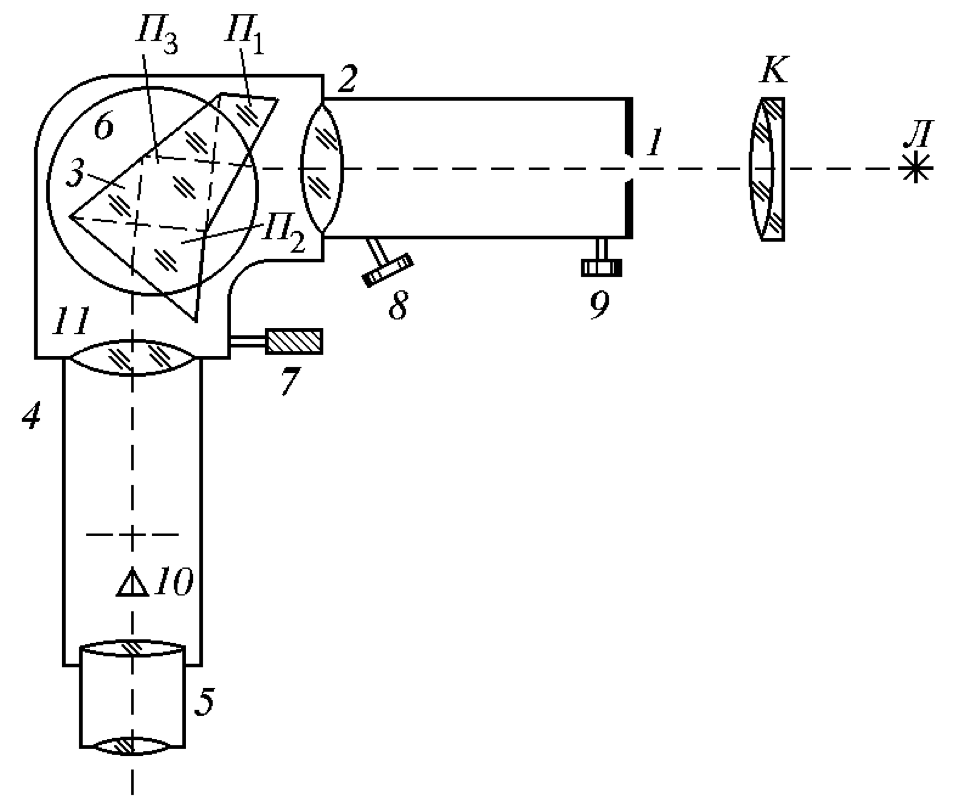
\includegraphics[width=10cm]{res/scheme.png}
		\caption{Устройство монохроматора УМ-2}
	\end{figure}
	Первые две призмы с преломляющими углами $30^\circ$ изготовлены из тяжелого флинта, обладающего большой дисперсией. Промежуточная призма П$_3$ сделана из крона. Лучи отражаются от ее гипотенузной грани и поворачиваются на $90^\circ$. Благодаря такому устройству дисперсии призм П$_1$ и П$_2$ складываются.
	
	Для отсчета положения спектральной линии ее центр совмещается с острием указателя. Отсчет проводится по делениям барабана.
	
	Для градуировки в коротковолновой части спектра удобно применять ртутную лампу ПРК-4, а в длинноволновой и средней части спектра -- неоновую лампу. 
	
	Для увеличения яркости интересующих нас линий атомарного водорода в состав газа, которым заполняют трубку при ее изготовлении, добавляют пары воды. Молекулы воды в электрическом разряде разлагаются, образуя атомарный водород. Трубка заполняется газом до давления 5–10 Тор.

	
    \section*{Ход работы}
	

 \begin{enumerate}
 
    \item Проградуируем спектрометр УМ-2 по спектрам неона и ртути. Отсчитываем угол по барабану. Погрешность измерения углов $\sigma_{\theta} = 5^\circ$. Результаты для неона и ртути запишем в таблицы \ref{HydrogenSpectre_GradsTableNeon} и \ref{HydrogenSpectre_GradsTableMercury}.

    \begin{table}[h!]
       \centering
       \footnotesize
       \begin{tabular}{ccc}
\toprule
\multicolumn{3}{c}{\text{Неон}}\\
\text{Линия} & \text{Угол}, $\theta ^\circ$ & \text{Длина волны}, \AA \\
\midrule
23 & 1846 & 5401 \\
22 & 2150 & 5852 \\
20 & 2196 & 5945 \\
15 & 2284 & 6143 \\
8  & 2390 & 6402 \\
4  & 2486 & 6678 \\
\bottomrule
\end{tabular}

       \caption{Градуировка по спектру неона}
       \label{HydrogenSpectre_GradsTableNeon}
    \end{table}

    \begin{table}[h!]
       \centering
       \footnotesize
       \begin{tabular}{ccc}
\toprule
\multicolumn{3}{c}{\text{Ртуть}}\\
\text{Линия} & \text{Угол}, $\theta ^\circ$ & \text{Длина волны}, \AA \\
\midrule
6  & 284  & 4047 \\
5  & 844  & 4358 \\
4  & 1506 & 4916 \\
3  & 1928 & 5461 \\
2  & 2108 & 5770 \\
K2 & 2324 & 6234 \\
K1 & 2556 & 6907 \\
\bottomrule
\end{tabular}

       \caption{Градуировка по спектру ртути}
       \label{HydrogenSpectre_GradsTableMercury}
    \end{table}

    Построим градуировочный график, основываясь на этих данных.

		
    \begin{figure}[h!]
        \centering
        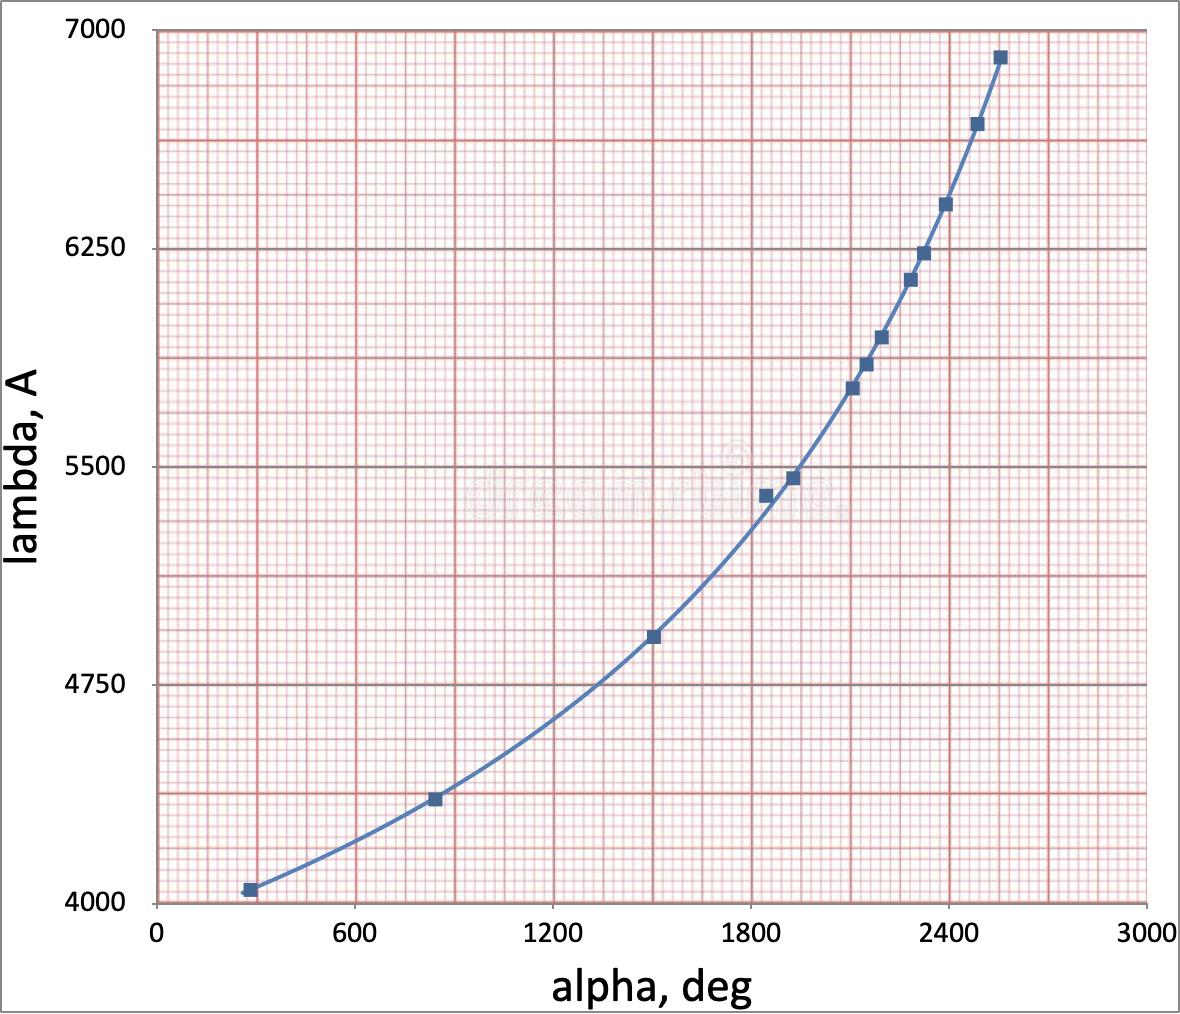
\includegraphics[width=10cm]{src/plotApprox.png}
        \caption{Зависимость $\lambda(\theta)$}
    \end{figure}

    Использовалась аппроксимация:
    \begin{equation*}
        \lambda(\theta) = A + \frac{B}{\theta - C}.
    \end{equation*}
    Из расчетов получаем следующее:
    \begin{itemize}
        \item $A = (2294 \pm 73)$ \AA
        
        \item $B = (-6440 \pm 307) \cdot 10^3$ \AA
        
        \item $C = (3956 \pm 48)$
        
    \end{itemize}
    
    \item Измерим положения линий атома водорода. Результаты пишем в таблицу \ref{HydrogenSpectre_LinesTable}.

    \begin{table}[h!]
       \centering
       \footnotesize
       \begin{tabular}{cc}
\toprule
\text{Линия} & \text{Угол}, $\theta ^\circ$ \\
\midrule
H_{\delta} & 388  \\
H_{\gamma} & 816  \\
H_{\beta}  & 1452 \\
H_{\alpha} & 2444 \\
\bottomrule
\end{tabular}

       \caption{Линии атома водорода}
       \label{HydrogenSpectre_LinesTable}
    \end{table}

	Используя аппроксимирующую формулу и градуировочный график, найдем значения длин волн для этих линий. Погрешность для каждой:
	\begin{equation*}
		\sigma_\lambda = \sqrt{\left(\frac{\partial \lambda}{\partial A}\right)^2 \sigma_A ^2 + \left(\frac{\partial \lambda}{\partial B}\right)^2 \sigma_B ^2 + \left(\frac{\partial \lambda}{\partial C}\right)^2 \sigma_C ^2 + \left(\frac{\partial \lambda}{\partial \theta}\right)^2 \sigma_\theta ^2}
	\end{equation*}
	\begin{equation*}
		\sigma_{\lambda} = \sqrt{\sigma_A^2 + \frac{\sigma_B^2}{(\theta - C)^2} + \frac{B^2 \sigma_C^2}{(\theta - C)^4} + \frac{B^2 \sigma_\theta^2}{(\theta - C)^4}}
	\end{equation*}

    \begin{table}[h!]
       \centering
       \footnotesize
       \begin{tabular}{cc}
\toprule
\text{Линия} & \text{Угол}, $\theta ^\circ$ \\
\midrule
H_{\delta} & 388  \\
H_{\gamma} & 816  \\
H_{\beta}  & 1452 \\
H_{\alpha} & 2444 \\
\bottomrule
\end{tabular}

       \caption{Сводная таблица по линиям атома водорода}
       \label{tab:t3}
    \end{table}

	Как видим, результаты чрезвычайно близки к табличным. Ошибка определения длин волн составляет $\thicksim 0.1-0.3\%$.

	\item Теперь рассчитаем постоянную Ридберга $R$ для каждой линии. Результаты в таблице \ref{HydrogenSpectre_RydbergTable}.

     \begin{table}[h!]
       \centering
       \footnotesize
       
\begin{tabular}{cccc}
\toprule
\text{Линия} & \text{Постоянная Ридберга} $R$, см$^{-1}$ & $1/n^2 - 1/m^2$ & $1/\lambda$, $10^{-4}$ \AA$^{-1}$\\
\midrule
H_{\delta} & 109774.242 & 0.222 & 2.439 \\
H_{\gamma} & 109585.092 & 0.210 & 2.301 \\
H_{\beta}  & 109593.813 & 0.188 & 2.055 \\
H_{\alpha} & 109848.408 & 0.139 & 1.526 \\
\bottomrule
\end{tabular}

       \caption{Значение постоянной Ридберга, рассчитанное по линиям водорода}
       \label{HydrogenSpectre_RydbergTable}
    \end{table}
	
	В среднем получаем:
	\begin{equation*}
		\boxed{R = (109700 \pm 100) \text{ см}^{-1}}  \iffalse 117 \fi
	\end{equation*}

	Попробуем задействовать сразу все линии, чтобы разово вычислить постоянную Ридберга.
	Построим график такой вот зависимости величин $\frac{1}{\lambda} = f\left(\frac{1}{n^2} - \frac{1}{m^2}\right)$ и по наклону найдем значение $R$. Поскольку $n$ и $m$ -- это целые числа, то погрешности по оси абсцисс нет. Вдобавок, мы знаем погрешность для каждого значения $1/\lambda$. Именно поэтому выбираем метод построения $\chi^2$.

	В нашем приближении: $1/\lambda = R \cdot \left(\frac{1}{n^2} - \frac{1}{m^2}\right)$.
	\begin{equation*}
		\chi^2 = \sum\limits_{i = 1}^4 \frac{(y_i - kx_i)^2}{\sigma_{y_i}^2} \rightarrow \min \Longrightarrow k = \dfrac{\sum\limits_{i = 1}^4 \dfrac{x_i y_i}{\sigma_{y_i}^2}}{\sum\limits_{i = 1}^4 \dfrac{x_i^2}{\sigma_{y_i}^2}}
	\end{equation*}

	\begin{figure}[h!]
		\centering
		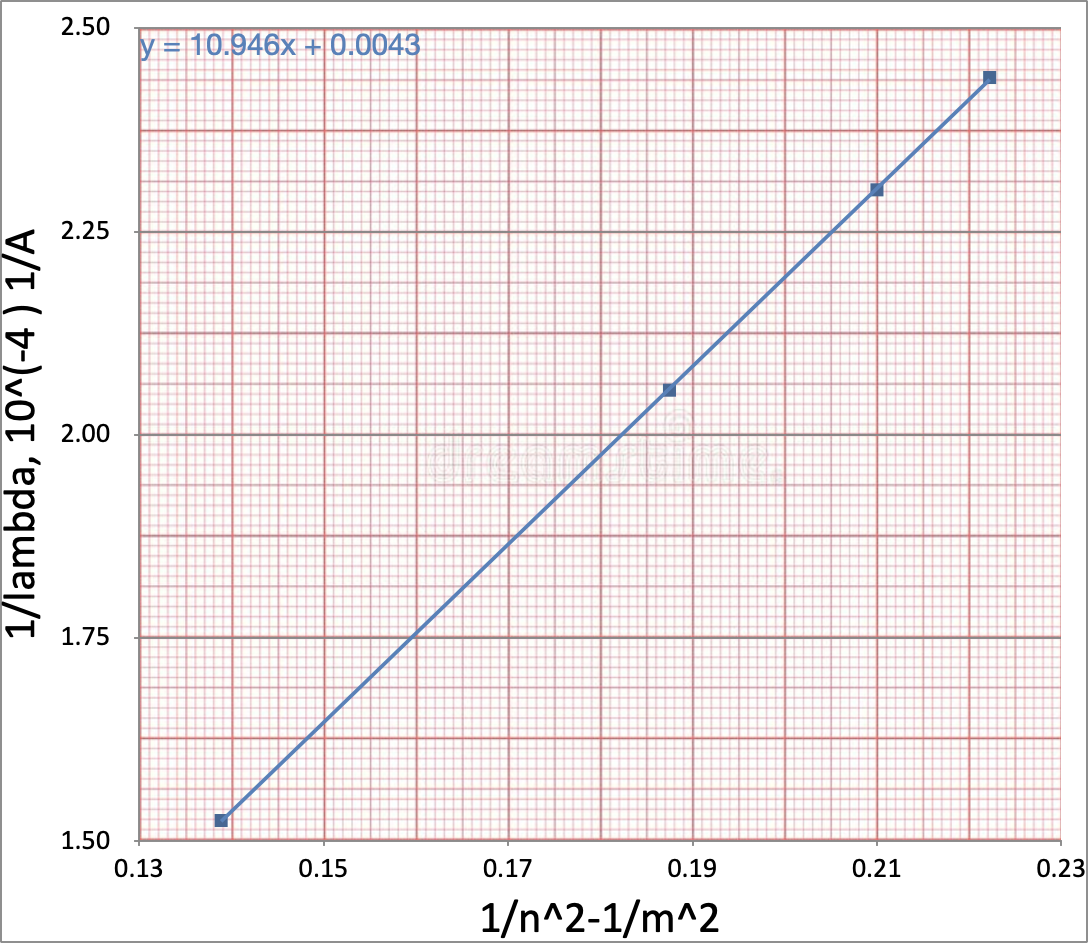
\includegraphics[width=10cm]{src/line.png}
		\caption{Зависимость $1/\lambda$ от $1/n^2 - 1/m^2$}
	\end{figure}

	Из графика получаем ($k = R$):
	\begin{equation*}
		\boxed{R = (109460 \pm 100) \text{ см}^{-1}}
	\end{equation*}

	То есть найденное только что значение находится в согласии с ранее посчитанными.
	Учитывая, что табличное значение $R = 109677.6$ см$^{-1}$, то можно сказать, что найденные результаты с отличной точностью совпадают как между друг с другом, так и с табличным значением. 

    \item Найдём длины волн для йода:

     \begin{table}[h!]
       \centering
       \footnotesize
       \begin{tabular}{ccc}
\toprule
 & \text{Угол}, $\theta ^\circ$ & \text{Длина волны} $\lambda$, \AA \\
\midrule
\nu_{1, 0} & 2354 & 6315 \pm 15 \\
\nu_{1, 8} & 2246 & 6061 \pm 10 \\
\nu_{гр}   & 1696 & 5144 \pm 10 \\
\bottomrule
\end{tabular}

       \caption{Измерения для йода}
       \label{IodTable}
    \end{table}

	Вычислим в электрон-вольтах энергию колебательного кванта возбуждённого состояния молекулы йода:
	\[h\nu_2 = 15 \;\text{МэВ}.\]
	
	Найдём параметры диссоциации молекул йода:
	\[h\nu_{\text{эл}} = h\nu_{1, 0}+\dfrac{3}{2}h\nu_1 - \dfrac{1}{2}h\nu_2 = 2.13\pm 0.03\; \text{эВ}.\]
	Эта величина получена из формулы \eqref{eq:iodine}. Тогда для энергии диссоциации частиц в основном и возбуждённом состояниях:
	\[D_1 = h\nu_{\text{гр}} - E_A = 1.48\pm 0.02\; \text{эВ},\]
	\[D_2 = h\nu_{\text{гр}} - h\nu_{\text{эл}} = 0.28\pm 0.02\; \text{эВ}.\]
	Здесь $ E_A = 0.94\; \text{эВ}$ -- энергия возбуждения атома.


    Энергии колебательного кванта возбуждённого состояния молекулы йода:
    \[h\nu_{2} = \dfrac{h\nu_{1,8} - h\nu_{1,0}}{8} = 0.010 \pm 0.005~\text{эВ}.\]
    Учитывая, что $h\nu_1 = 0.027~\text{эВ}$, с помощью формулы (2) рассчитаем энергию перехода
    \[h\nu_{\text{эл}} = h\nu_{1,0} - \dfrac{1}{2} h\nu_2 + \dfrac{3}{2} h\nu_1 = 2.00 \pm 0.03~\text{эВ}.\]
    Тогда энергии диссоциации частиц в основном и возбуждённом состоянии, с учётом того, что энергия возбуждения атома $E_A = 0.94~\text{эВ}$:
    \[D_1 = h\nu_{\text{гр}} - E_A = 1.47 \pm 0.02~\text{эВ},\]
    \[D_2 = h\nu_{\text{гр}} - h\nu_{\text{эл}} = 0.41 \pm 0.07~\text{эВ}.\]

	\end{enumerate}

	\section*{Вывод}
    \begin{itemize}
        \item Экспериментально проверена справедливость формулы Бальмера и найдена постоянная Ридберга $R = 109700 \pm 100 \;
        \text{см}^{-−1} $, которая в пределах погрешность совпадает с табличной $ R_\text{табл} = 109700.6  \; \text{см}^{-−1} $
        \item Оценена энергия квантов возбужденного состояния молекулы, энергия диссоциации частиц и энергия электронного перехода.
    \end{itemize}

\newpage
\begin{thebibliography}{9}
	\bibitem{max} \emph{Лабораторный практикум по общей физике. В 3 томах. Том 3. Квантовая физика: учебное пособие} под ред. Ю. М. Ципенюка
\end{thebibliography}

\end{document}
